\section{The Exocentric vision issue}
\label{sec:exo}
\subsection{Why use exocentric vision?}
Teleoperated mobile robots prove to be extremely useful 
when there is the need for performing operations in places that 
are unaccessible or dangerous for human beings - e.g. 
search-and-rescue missions within unknown regions or into 
collapsed buildings, caves, etc.
%
The supervisors' research group has been widely involved 
during the last years in the research on teleoperated robots. 
[citation needed].

As for the testing platform, they have been using 3morduc,
a differential-drive mobile robot - showed in figure \ref{fig:morduc} -
equipped with a pair of Videre Design [citation needed] 
stereo cameras and a laser scanner.
They have been focused on the making of a reliable software 
infrastructure which makes able a remote operator to drive 
the 3morduc in a comfortable fashion.
%% parlare dei campi di ricerca coinvolti?
%
\begin{figure}[!h]
  \begin{center}
    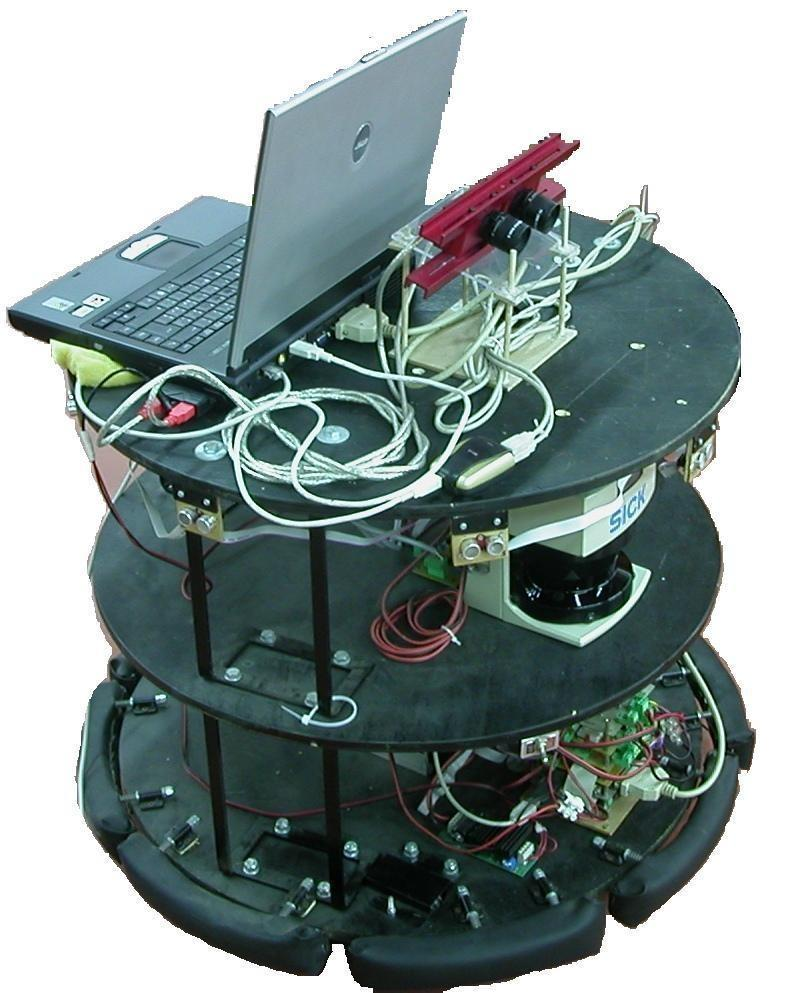
\includegraphics[width=200pt]{img/3morduc}  %robot pic
    \caption{The 3morduc robotic platform}
    \label{fig:3morduc}
  \end{center}
\end{figure}
%
[Indeed],our work focused on the robot-operator interaction and, 
hence, on how to improve such interaction. Analyzing previous work 
and data produced by the supervisors' research group, it emerges 
that the stereo cameras mounted on top of 3morduc, were used to 
provide the remote operators a \textit{first-person} point of view. 
In literature, such a system is also called an \textit{egocentric} 
vision system.
%

%
According to \cite{sugimoto}, \textit{by observing the camera image 
without an efficient human interface system, the operator 
tends to misinterpret the robot's position and direction}. This is 
due to the fact that  \textit{it's difficult for an
operator not accustomed to the vehicle to estimate the
vehicle's position and direction and the distances to a
target strictly based on camera images from the firstperson 
viewpoint}.
%
In order to improve the interaction between the robot and the operator 
an exocentric camera would be effective since it would provide a 
representation of the robot in the operating environment and, thus, 
a better understanding of where the robot is located into the environment 
and its actual direction.
%
Unfortunately the use of an exocentric camera is not trivial: for example, 
it could be mounted on a [dedicated long support] on the back of the robot, 
but such a support would terribly disturb the robot activity and its 
moving abilities. [di fatto e` un vincolo in piu` che si sta aggiungendo]
%
Non solo, una immagine precedente, contiene informazioni ambientali piu' 
ampie rispetto a quelle di una camera montata sul posteriore del robot.
%
To avoid such complications, \cite{sugimoto} proposes 
\textit{Time Follower's}, an approach to provide a virtual exocentric 
view.
%
%
\subsection{Time Follower's: an overview}
Time Follower's aims at providing an exocentric view of a mobile 
robot using an egocentric-mounted camera. The approach is simple: it is 
based on the use of previously recorded first-person images to provide 
comprehensible third-person imagery. A 3D representation of the robot 
is overlapped to such images in order to get the work done.
%
Key issueof the system are:
\begin{itemize}
\item how to choose the \textit{best} image
\item how to determine the \textit{right} place to draw the robot
\end{itemize}
%
    [a brief description of the two concepts]
%

